% include the figures path relative to the master file
\graphicspath{ {./content/method/figures/} }

\section{\replaced[id=sik]{Experimental Setup}{Materials and Methods}}\label{sec:method}\label{sec:exp}
The experimental set-up is formulated as a standard classification procedure consisting of 5 steps.
Figure~\ref{fig:ML-scheme} outlines these 5 steps and illustrates how the methodologies have been translated to such schema.

\begin{figure*}
  \centering{
    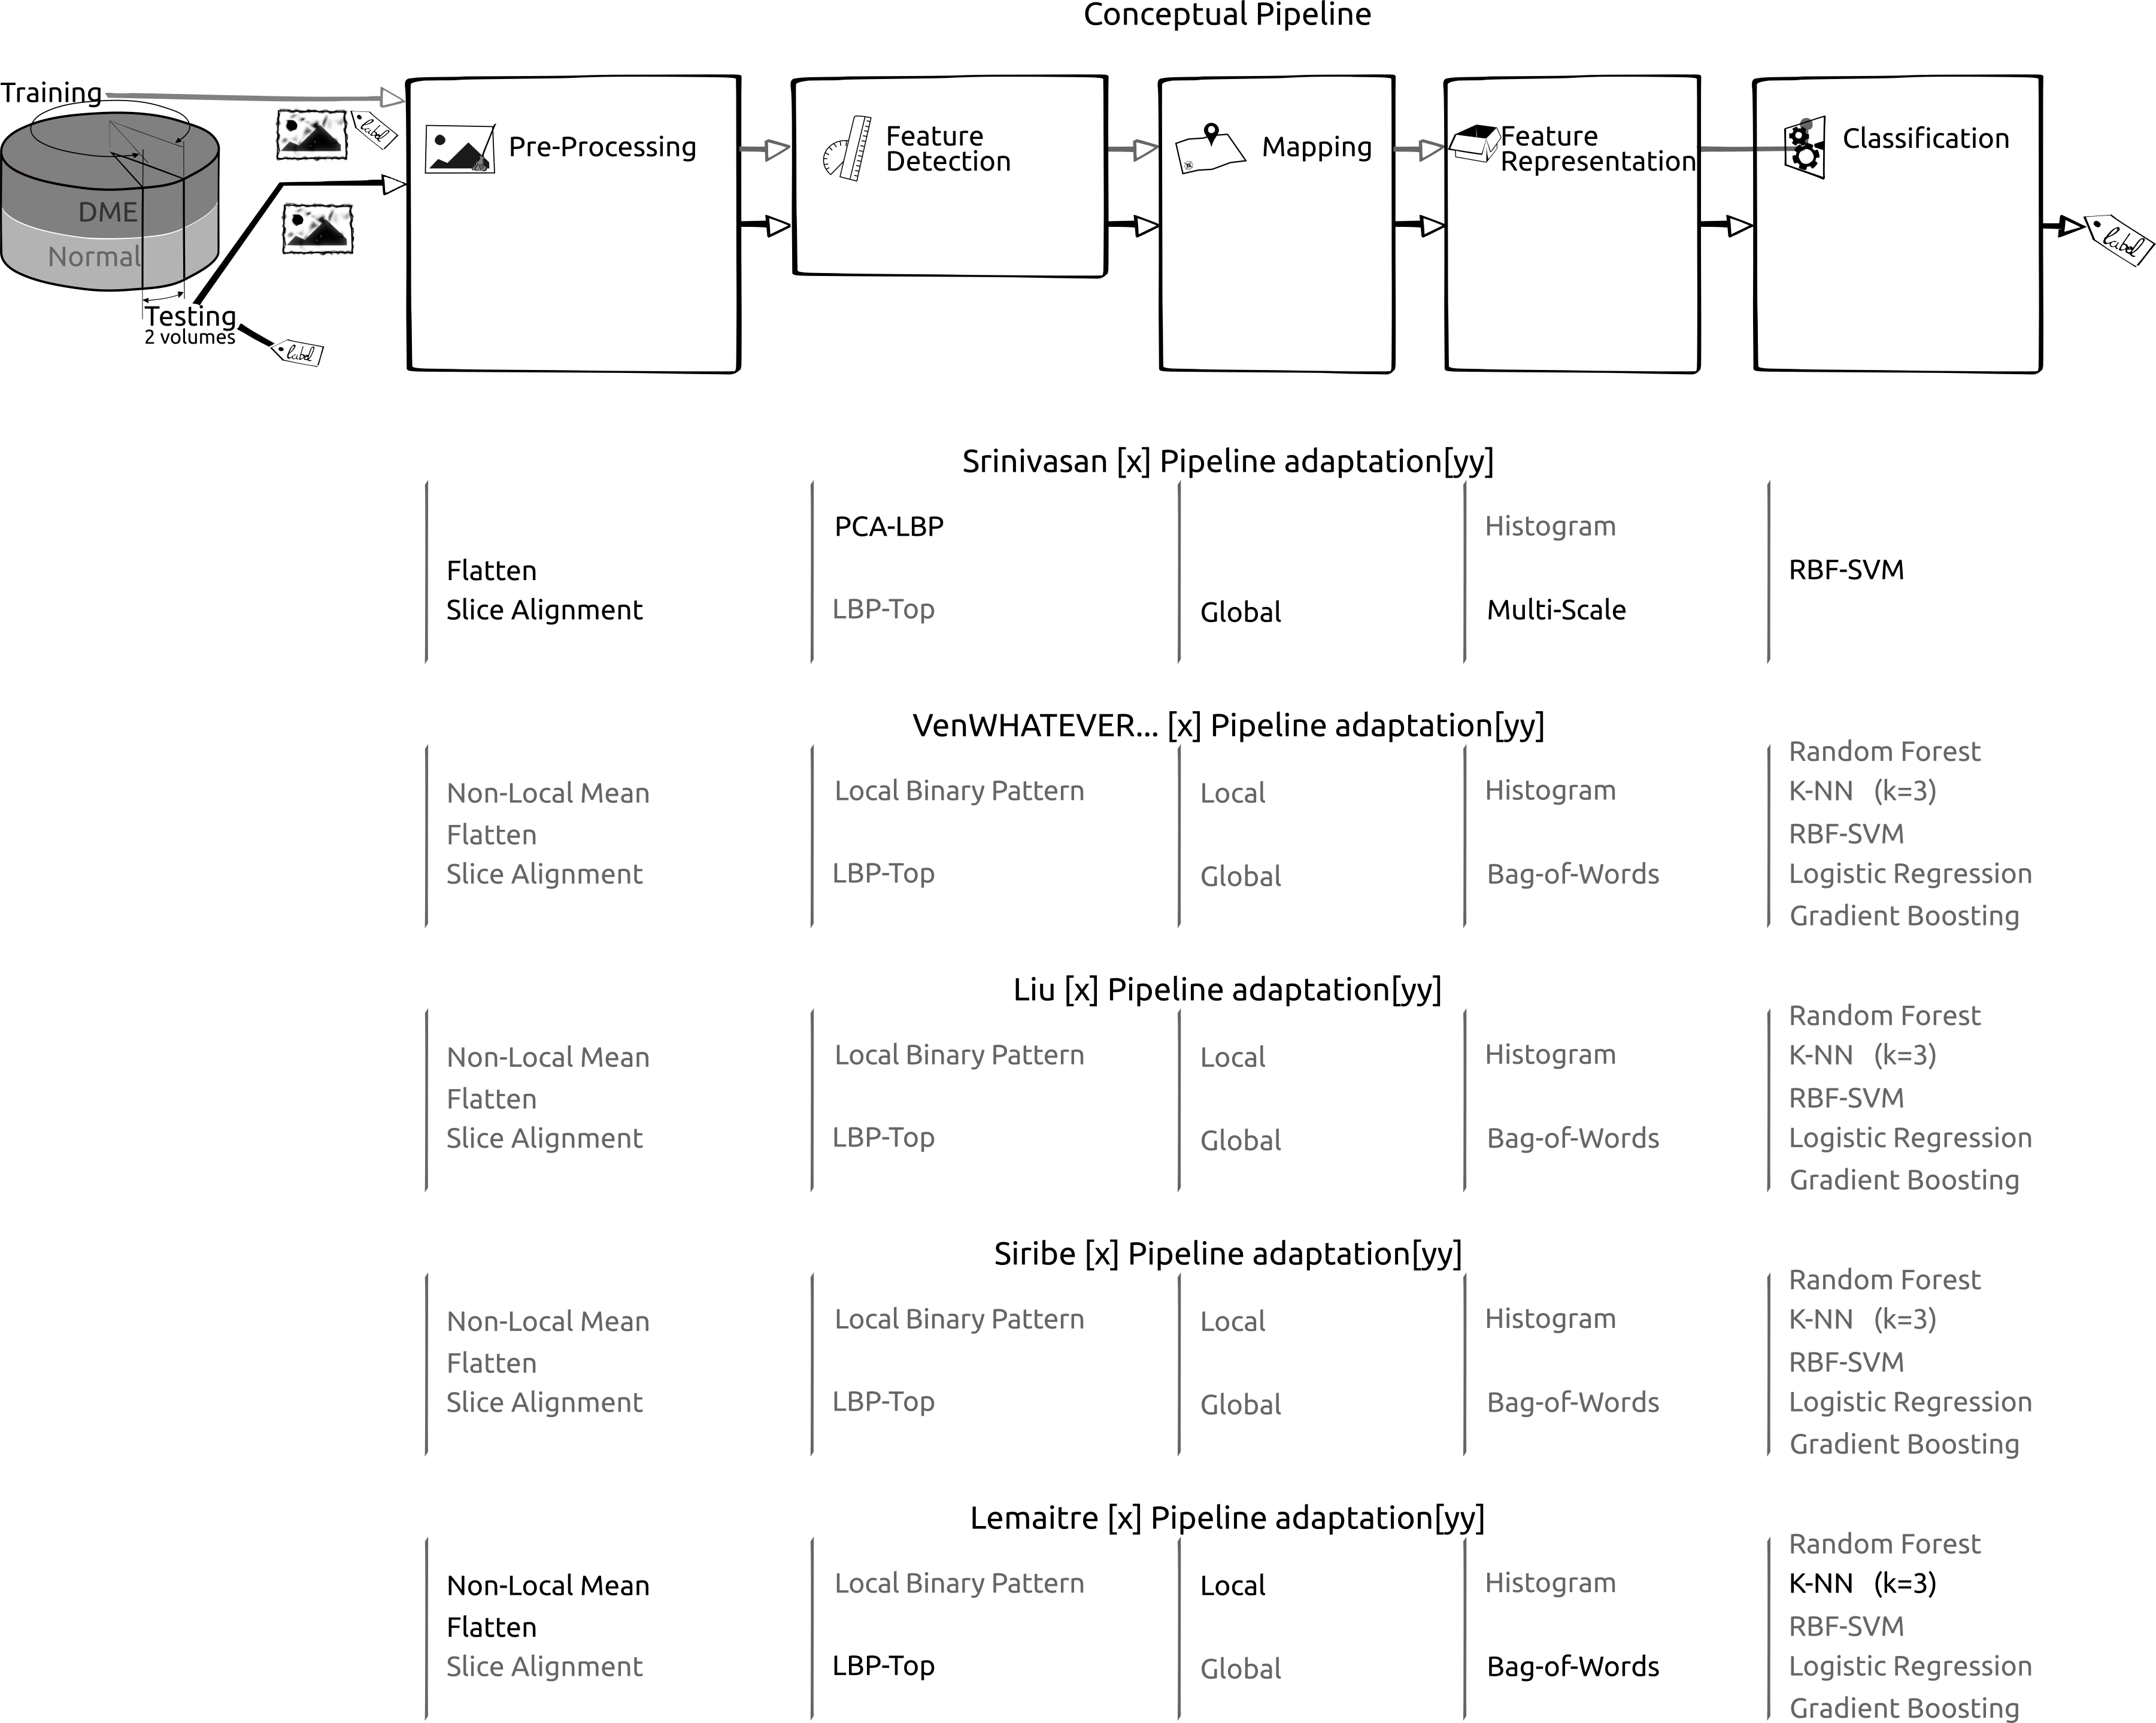
\includegraphics[width=1\linewidth]{ml}}
    \caption{Experimental Setup}
  \label{fig:ML-scheme}
\end{figure*}

\subsection{\deleted[id=sik]{method comments}}
\todo[inline]{here goes a description left to right of the modules, making remarks of the difference between the needs of each method.}
\added[id=old]{
First, the \gls{oct} volumes are pre-processed as presented in details in Sect.\,\ref{subsec:prepro}.
%Then toward a final descriptor \gls{lbp} and \gls{lbptop} features are extracted with different mapping strategy and represented using two approach.
Then, \gls{lbp} and \gls{lbptop} features are detected, mapped and represented as discussed in depth in Sect.\,\ref{subsec:feaext}, Sect.\,\ref{subsec:mapping}, and Sect.\,\ref{subsec:fearep}, respectively.
%{\color{red}The feature extraction, mapping, and representation are presented in depth in Sect.\,\ref{subsec:feaext}, Sect.\,\ref{subsec:mapping}, and Sect.\,\ref{subsec:fearep}, respectively. CHECK THE SECTION ORDERING}
Finally, the classification step is presented in Sect.\,\ref{subsec:cls}.
}

\deleted[id=sik]{The mapping in A is computed in this manner while in B this comes on the other side bla bla bla}

\subsection{Data}\label{sec:exp:data}
\deleted[id=sik]{
  Despite Venhuizen et al. tested on a public dataset~\cite{dukeBIG}, this dataset is intended to AMD.
  Srinivasan also tested on a public dataset~\cite{dukeSmall}, however the images are cropped and filtered etc.
  So thats why we collected the SERI dataset.
}

\added[id=old]{
This dataset was acquired by the Singapore Eye Research Institute (SERI), using
CIRRUS TM (Carl Zeiss Meditec, Inc., Dublin, CA) \gls{sdoct} device. The dataset
consists of 32 \gls{oct} volumes (16 \gls{dme} and 16 normal cases). Each volume
contains 128 B-scan with resolution of 512 $\times$ 1024 pixels.  All
\gls{sdoct} images are read and assessed by trained graders and identified as
normal or \gls{dme} cases based on evaluation of retinal thickening, hard
exudates, intraretinal cystoid space formation and subretinal fluid.
}

\subsection{Validation}\label{sec:exp:validation}
\added[id=old]{
All the experiments are evaluated in terms of \gls{se} and \gls{sp} using the \gls{lopocv} strategy, in line with \cite{Lemaintre2015miccaiOCT}.
\gls{se} and \gls{sp} are statistics driven from the confusion matrix (see Fig.\,\ref{fig:CM}) as stated in Eq.\,\eqref{eq:sesp}.
The \gls{se} evaluates the performance of the classifier with respect to the positive class, while the \gls{sp} evaluates its performance with respect to negative class.
}
\begin{align}
 \gls{se}  = \frac{TP}{TP+FN} \qquad \gls{sp} = \frac{TN}{TN+FP}
 \label{eq:sesp}
\end{align}
\added[id=old]{
The use of \gls{lopocv} implies that at each round, a pair \gls{dme}-normal volume is selected for testing while the remaining volumes are used for training.
Subsequently, no \gls{se} or \gls{sp} variance can be reported.
However, \gls{lopocv} strategy has been adopted despite this limitation due to the reduced size of the dataset.
}

\subsection{Management of data depending terms}
\deleted[id=sik]{
  Be aware that when computing the GMM~\cite{repo_des}, or the dictionary
  \cite{repo_lem}, only the training data for the current fold is used.
  Therefore such modules are recomputed at each fold.
}
\deleted[id=sik]{
  Other parameter tuning such the case of XXXX and YYYYY are also carried out using only ZZZZ
}
